\documentclass[border=10pt]{standalone}
\usepackage{tikz}
\usetikzlibrary{automata, positioning, arrows.meta}

\begin{document}
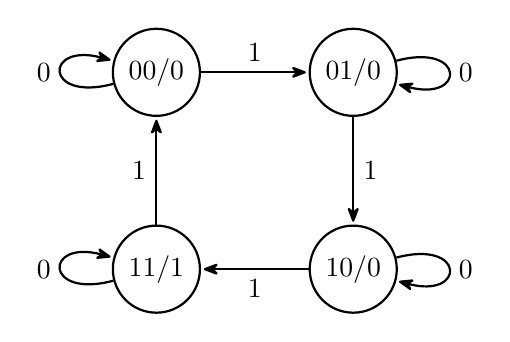
\begin{tikzpicture}[shorten >=1pt, node distance=2.5cm, on grid, auto, >={Stealth[round]}, thick]
    % Nodes (Moore: State/Output)
    \node[state] (s00) {00/0};
    \node[state] (s01) [right=of s00] {01/0};
    \node[state] (s11) [below=of s00] {11/1};
    \node[state] (s10) [below=of s01] {10/0};

    % Transitions
    % 00 -> 00 (0), 01 (1)
    % 01 -> 01 (0), 10 (1)
    % 10 -> 10 (0), 11 (1)
    % 11 -> 11 (0), 00 (1)
    \path[->]
        (s00) edge [loop left] node {0} (s00)
              edge node {1} (s01)
        (s01) edge [loop right] node {0} (s01)
              edge node {1} (s10)
        (s10) edge [loop right] node {0} (s10)
              edge node {1} (s11)
        (s11) edge [loop left] node {0} (s11)
              edge node {1} (s00);
\end{tikzpicture}
\end{document}
